\subsection{Origin of a solarsystem}
In the first stage of galaxy building the matter that will later be our galaxy is a Protosolar fog with a huge diameter of 20000 \ac{AU}. \ac{AU} is the distance between the earth and the sun. After some time the fog collapsed under its own gravitational pull resulting in an increase in density. We call this stage protoplanetary disk with an diameter of about 200 \ac{AU}. Over time the dust formed to bigger and bigger chuncks due to gravity. So the planets were formed.\\ The cause why the terrestrial planets formed closer to the sun was that the temperature at the inner planets (Mercury, Venus, Earth, and Mars)) was to high to keep volantile molekules to them. Just heavy atoms like iron, nickel, and aluminum. The outer planets (Jupiter, Saturn, Uranus, and Neptune) were able to collect more volantile molekules resulting in much bigger size. The last stage that we encoutered was the \ac{LHB} which is a time in which the moon and the earth was hit by a lot of Meteors.

\subsection{Geography of our Solar system}
A picture of our solar system can be found in figure \ref{fig:Foliensatz1:geography}. Ein Merksatz für unser Sonnensystem ist: Unser Vater erklärt mir jeden Sonntag unsere neun planeten. While we only have eight planets. Pluto is a Dwarf planet
\begin{figure}
    \centering
    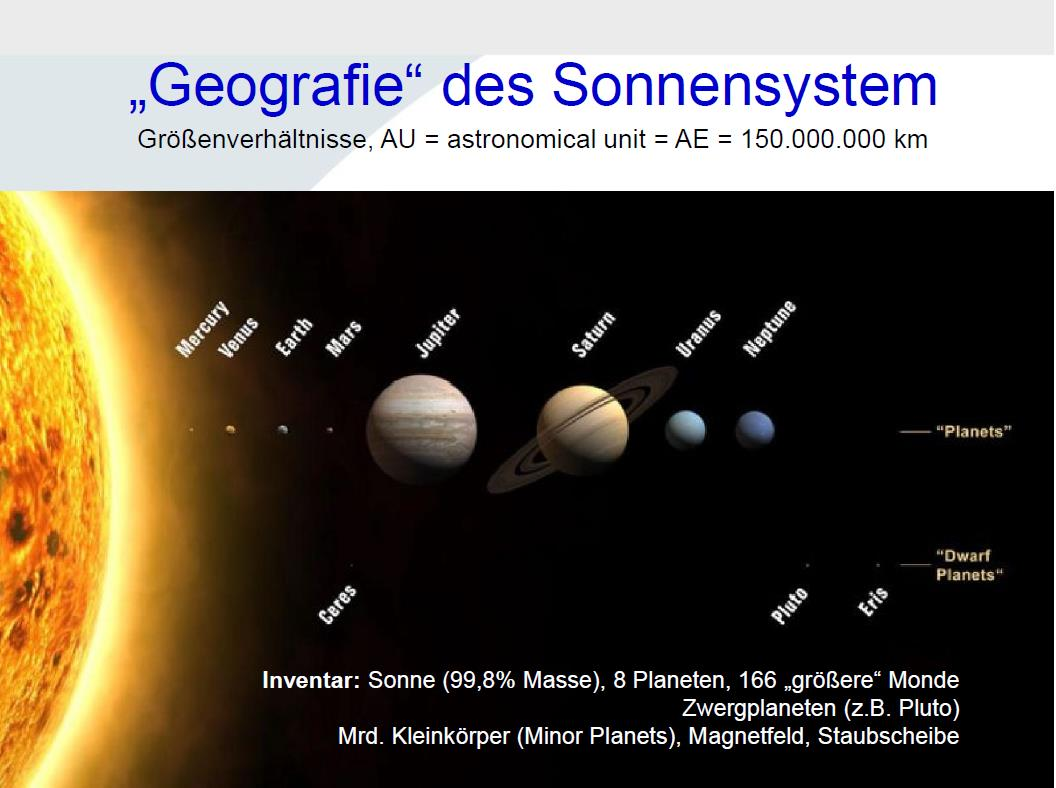
\includegraphics[width=0.7\textwidth]{images/Foliensatz1_geography_of_our_solarsystem.png}
    \caption{A picture of our Solarsystem}
    \label{fig:Foliensatz1:geography}
\end{figure}

\subsection{Definitons}
\subsubsection{What is a Planet}
A celestial body is a planet if it fullfills the following points:
\begin{enumerate}
    \item If it orbits around the sun\\
    \item It needs suffiecient mass for its self-gravity to overcome rigid body forces so that it asumes hydrostatic equilibrium (almost round shape)
    \item Hast cleared its neighbourhood from debre and other foreign bodies
\end{enumerate}
\subsubsection{What is a dwarf planet}
A Dwarf Planet is a new class of Celestial body of which pluto is the prime example. In comparison to a planet it can still have trash and other objects in it orbit that means a Dwarf planet is a dwarf planet if it fullfills the following points:
\begin{enumerate}
    \item If it orbits around the sun\\
    \item It needs suffiecient mass for its self-gravity to overcome rigid body forces so that it asumes hydrostatic equilibrium (almost round shape)
    \item Has not cleared its neighbourhood from debre and other trash yet
    \item and it needs to not be a Satellite
 \end{enumerate}   
\subsubsection{Small Solar-system Bodies}
Are all other bodies orbiting the sun except satellites

\subsubsection{Other celestial bodies that need to be distinguised}
\begin{enumerate}
    \item  Komet\\
    A big pile of rock orbiting the sun.
    \item Asteroid\\
    smaller pile of rock that orbits the sun
    \item Meteroride\\
    Even smaller object flying through space orbiting the sun. The size is between meters and $\mu$ meters.
    \item Meteor\\
    A Meteoride hitting earth but burning up in the athmosphere
    \item Meterorite\\
     A meteor that hits Earth without burning up in the atmosphere
\end{enumerate}

\subsubsection{The interplanetary medium}
It consists of the following particles. First dust, cosmic rays from \ac{SN}, \ac{BH} and neutron-stars. Additonally there are magnetic fields and Sunwinds.

\subsection{The scattered disk}
The scattered disk is assortment of millions of comets with different rings. The innermost being the Kuiper Nelt. It is thought that this might be the cause for the amount of regular comets we see. The comets have a broad band with of eccentricities and inclination. The whole Comet belt is called the Oort Cloud and is a cloud around our solar system.



